\documentclass[review]{elsarticle}
%\documentclass[final,8pt,authoryear,twocolumn]{elsarticle}

%% Use the option review to obtain double line spacing
%% \documentclass[preprint,review,12pt]{elsarticle}

%% Use the options 1p,twocolumn; 3p; 3p,twocolumn; 5p; or 5p,twocolumn
%% for a journal layout:
%% \documentclass[final,1p,times]{elsarticle}
%% \documentclass[final,1p,times,twocolumn]{elsarticle}
%% \documentclass[final,3p,times]{elsarticle}
%% \documentclass[final,3p,times,twocolumn]{elsarticle}
%% \documentclass[final,5p,times]{elsarticle}
%% \documentclass[final,5p,times,twocolumn]{elsarticle}

%% if you use PostScript figures in your article

%% or use the graphicx package for more complicated commands
\usepackage{graphicx}
\graphicspath{{Figures/}}
%% or use the epsfig package if you prefer to use the old commands
\usepackage{epsfig}
%% The amssymb package provides various useful mathematical symbols
\usepackage{amssymb,amsmath}
%% The amsthm package provides extended theorem environments
\usepackage{amsthm}
\usepackage{algorithm}
\usepackage{algpseudocode}
\usepackage{textcomp}
\usepackage{subcaption}


%% The lineno packages adds line numbers. Start line numbering with
%% \begin{linenumbers}, end it with \end{linenumbers}. Or switch it on
%% for the whole article with \linenumbers after \end{frontmatter}.
%\usepackage{lineno}

%% natbib.sty is loaded by default. However, natbib options can be
%% provided with \biboptions{...} command. Following options are
%% valid:

%%   round  -  round parentheses are used (default)
%%   square -  square brackets are used   [option]
%%   curly  -  curly braces are used      {option}
%%   angle  -  angle brackets are used    <option>
%%   semicolon  -  multiple citations separated by semi-colon
%%   colon  - same as semicolon, an earlier confusion
%%   comma  -  separated by comma
%%   numbers-  selects numerical citations
%%   super  -  numerical citations as superscripts
%%   sort   -  sorts multiple citations according to order in ref. list
%%   sort&compress   -  like sort, but also compresses numerical citations
%%   compress - compresses without sorting
%%
%% \biboptions{comma,round}

% \biboptions{}
\usepackage{hyperref}
\usepackage{color}
\usepackage{textcomp}
\usepackage{multirow}
\usepackage{float}
\usepackage{amsmath}
\usepackage{lineno}
\usepackage{color,soul}

\journal{Computer and Chemical Engineering}

\begin{document}

\begin{frontmatter}
\title{Accelerating multi-dimensional population balance model simulations via a highly 
scalable framework using GPUs.}


\author[label1]{Chaitanya Sampat}
\author[label1]{Yukteshwar Baranwal}
\address[label1]{Chemical and Biochemical Engineering, 
Rutgers University, Piscataway, NJ, USA - 08854}
\author[label1]{Rohit Ramachandran\corref{cor1}}
\ead{rohitrr@soemail.rutgers.com}
\cortext[cor1]{Corresponding author}
%\ead[url]{pslrutgers.com}

\begin{abstract}
The solution of high-dimensional PBMs using CPUs are often 
computationally intractable. This study focuses on the development of a scalable 
algorithm to parallelize the nested loops inside the PBM via a GPU framework. 
The developed PBM is unique since it adapts  to the size of the problem and uses 
the GPU cores accordingly. This algorithm was parallelized for
 NVIDIA\textsuperscript{\tiny\textregistered} GPUs as it was written in 
 CUDA\textsuperscript{\tiny\textregistered} and C/C++. The major 
bottleneck of such algorithms is the communication time between the CPU and the GPU. 
In our studies, communication time contributed to less than 1\% of the total run 
time and a maximum speedup of about 12 over the \hl{serial CPU code was achieved}. 
The GPU PBM achieved a speedup of about two times compared to the PBM's
multi-core configuration on a desktop computer. The speed improvements are also 
reported for various CPU \& GPU architectures and configurations.

\end{abstract}

\begin{keyword}
%% keywords here, in the form: keyword \sep keyword
Population Balance Model \sep GPU \sep Parallel Computing \sep Granulation \sep MPI \sep CUDA
%% MSC codes here, in the form: \MSC code \sep code
%% or \MSC[2008] code \sep code (2000 is the default)
\end{keyword}

\end{frontmatter}

\begin{linenumbers}
%% main text
\section{Introduction}
\label{secIntro}
Various chemical industries such as detergent, food, pharmaceutical, fertilizers, catalyst 
deal with particulate processing on a daily basis. These processes constitute to about 
$50\%$ of the world's chemical production \citep{seville1997}.
In the pharmaceutical industry, particulate processes are widely used to increase 
the size of the granules, improve flow-ability, increase yield strength etc. One of 
major processes is granulation, in which fine pharmaceutical powder 
blends are converted to larger granules using a liquid or a dry binder \citep{Chaturbedi2017}. 
These larger granules help in better flow ability and strength to these mixtures 
aiding further processing. 

Over the past decade, Population balance models (PBMs) have been used widely to predict 
dynamics of distributed processes \citep{ramkrishna2014}. The population 
balance equation is essentially a number conservation of particles (entities) which 
regulate the behavior of the entire particulate system. PBMs consist of several 
external (i.e spatial) and internal coordinates and with an increase in grids of 
these coordinates it can lead to a more accurate model.  With \hl{the} increase in 
the number of grid of these coordinates, it 
leads to an increase in calculations for each time step, leading to higher 
simulation times. The calculations increase by a factor of $n^4$ with n being the 
number of entity grids. PBMs describe the evolution of entities into different states and 
into newer entities. Deriving accurate equations to determine these rate of change 
of internal coordinates requires precise empirical correlations from 
experimental data. Another way to increase the accuracy of these models 
is to introduce a first-principle based kernel into these models \citep{Barrasso2015cerd}. 
An accurate model which incorporates higher number of grids as well as includes a 
mechanistic kernel in its calculations is expected to be \hl{sluggish} to simulate and could 
take upto an hour \citep{Barrasso2015ces} to complete. Such models and their 
solution techniques are not viable to be used in real time process control. Thus, 
there is a need to improve the time it takes to simulate a PBM. \hl{Thus, a highly parallel
PBM code which can predict more accurately in real time could be chosen over reduced order 
models currently used for process control.}

The advancement of computers and their peripherals in recent years have led to an  
increase in computational resources leading to faster simulations. The central processing 
units (CPUs) now contain multiple cores thus making it possible to run multiple processes 
in parallel. In order to take advantage of a highly parallel framework, large number of 
cores are required  which may not be possible in a personal desktop and a supercomputer 
cluster would be needed. Another computer component that can to be used to run a highly 
parallel code is the computer's graphic processing unit (GPU)~\citep{Prakash2013b}. 
These GPUs contain thousands of compute cores that can be used to run tasks in parallel. 
Thus, a GPU-equipped desktop could have compute power on par with a multi-CPU node
supercomputer. With the launch of Compute Unified Device Architecture 
(CUDA\textsuperscript{\tiny\textregistered}), 
NVIDIA\textsuperscript{\tiny\textregistered} made it easier to use GPUs for 
general parallel programming in an approach usually termed as general purpose computing on GPUs.

The main objective of this work is to develop a highly scalable framework for to simulate 
PBMs on GPUs. This framework is independent of the type of kernels as well as number 
of spatial compartments as well as the number of solid bins used. The framework is
universal and is able to run of different NVIDIA GPUs without the need for any changes. 
The number of threads that the PBM executes depends upon the size of the problem as well as 
the number of cores available on the GPU. This code was developed in 
NVIDIA\textsuperscript{\tiny\textregistered} 
CUDA\textsuperscript{\tiny\textregistered} C/C++. 
A similar code was also developed on C++ to be run on the CPU which has limited scalability 
due to number of CPU cores available on desktop computer. This work also enables the use of 
desktop computers to obtain numerical solutions to computationally intensive tasks rather 
than relying on supercomputers for quicker results.


\section{Background and previous works}
\label{secBkgd}
\subsection{Population balance modeling and wet granulation}

Population balances equations have been successful in 
predicting physical phenomena occurring in granulation such as aggregation, breakage and 
consolidation. These models predict how groups of distinct entities  behave on a bulk 
scale during granulation. A general representation of the model is:

\begin{align}
\frac{ \partial}{\partial t}&F(\textbf{v},\textbf{x},t) + \frac{\partial}{\partial 
\textbf{v}}[F(\textbf{v},\textbf{x},t)\frac{d\textbf{v}}{dt}(\textbf{v},\textbf{x},t)] 
+ \frac{\partial}{\partial \textbf{x}}[F(\textbf{v},\textbf{x},t)\frac{d\textbf{x}}{dt}
(\textbf{v},\textbf{x},t)] \notag\\
    &= 
\Re_{formation}(\textbf{v},\textbf{x},t)+\Re_{depletion}(\textbf{v},\textbf{x},t)
+\dot{F}_{in}(\textbf{v},\textbf{x},t) -\dot{F}_{out}(\textbf{v},\textbf{x},t) 
\label{eqn:bkgd_pbm_general} 
\end{align}

where $\textbf{v}$ is a vector of internal 
coordinates.  $\textbf{v}$ is commonly used to describe the solid, liquid, 
and gas content of each type of particle. The vector $\textbf{x}$ represents 
external coordinates, usually spatial. $F$ represents the 
number of particles present inside the system, $\dot{F}_{in}$ 
and $\dot{F}_{out}$ is the rate of particles coming in and going out the 
system respectively. $\Re_{formation}$ and $\Re_{depletion}$ are the rate of 
formation and depletion due various phenomena. $\Re_{formation}$ described in Equation 
\ref{eqn:mthds_R_agg} is the most computationally intensive component of the PBM.
This calculation consists of a double integral for each entity being tracked. In a 
system tracking 2 particulates, it would require 4 nested loops to compute these 
integrals. Figure \ref{fig:res_profile_pie} also indicates that this calculation 
takes $~25\%$ of the total run time. Thus, parallelizing this calculation \hl{is} crucial 
to the effectiveness of the parallel algorithm.

Wet granulation is the process of engineering granules from pharmaceutical powder blends 
with the addition of liquid or solid binders. This process is usually carried out 
to obtain granules with a certain PSD,  bulk densities and other physical properties
~\citep{Barrasso2015cerd}. There are about three rate processes that occur due the addition 
of a liquid binder to the powder mixture are wetting and nucleation, consolidation and 
aggregation, and breakage and attrition~\citep{sen2014}. One way to perform wet
granulation of pharmaceutical powders is to use a high shear granulator. 
In a high shear granulator, as the liquid binder is distributed within the granulator, 
liquid bridges are formed between particles and are subjected to the impeller. 
The impeller rotation along with particle-particle and particle-wall interactions 
results in the aforementioned granulation mechanisms.


\subsection{Parallel Computing}
Due to widely available access to high performance computing infrastructure, 
parallel computing has been extensively used by scientists to perform simulations. 
Parallel computing is the process of splitting of larger calculations into 
many smaller ones which can be executed concurrently \citep{Almasi1989}. This type of execution 
helps achieve large speed gains over serially running a simulation serially 
on a single core in a serial manner. \hl{The} computational task can be decomposed in two way, either
at the task level or at the data level. Task parallelism requires each process to 
behave distinctively from another as they would each be performing different operations. 
These operations could be performed on a single data set or on multiple data 
sets, known as multiple instructions single data (MISD) and multiple instructions 
multiple data (MIMD) respectively. On the other hand, data parallelism 
involves the distribution of data across various processes that usually perform same set of 
operations on the data \citep{solihin2015}. This type of parallelism is known 
as single instruction multiple data (SIMD). MIMD and SIMD can also 
be combined in certain systems, further reducing the simulation times.

\subsection{GPU based parallel computing}
Traditionally, large parallel jobs were run on supercomputers having thousands 
of cores, but these require special components making them expensive.
Graphic processing units (GPU) were initially used for vector calculations to support 
graphics inside a computer system. But, lately GPU manufacturers have started to promote their use in 
general computing as well. This form of GPU-based computing has been gaining popularity among scientists 
to accelerate simulations \citep{kandrot2011}. GPUs comprise of a 
massively parallel architecture with hundreds to thousands of computational cores 
which can have thousands of active threads running simultaneously \citep{keckler2011}. 
This means that GPUs have large computing potential which can be exploited using parallel 
programming languages such as OpenCL and CUDA\textsuperscript{\tiny\textregistered}. 

CUDA\textsuperscript{\tiny\textregistered} is an application programming interface 
(API) developed by NVIDIA\textsuperscript{\tiny\textregistered} \citep{NVIDIA2012} 
that enables users to program parallel code for execution on the GPU. Parallel code 
for the GPU is written as kernels, which are similar to functions or methods in traditional 
programming languages. As several parts of the code need to \hl{be} executed only once during a 
simulation, only a few sections of the code need to be written in terms of kernel while 
the remaining sections have to be serially executed on the CPU of the system. The \texttt{nvcc} 
compiler from the CUDA\textsuperscript{\tiny\textregistered} toolkit prioritizes the 
compilation of these kernels before passing the serial section of the code to the native 
C/C++ compiler inside the system. There are three main parallel abstractions that exist in 
CUDA\textsuperscript{\tiny\textregistered} viz. grids, blocks and threads \citep{santos2013}. 
Each kernel executes as a grid which in turn consists of various blocks which 
are consistuted by various threads. This thread-block-grid hierarchy helps obtain fine 
grained data level and thread level parallelism. An illustration of this hierarchy is 
observed in Figure \ref{fig:bkg_gpu_arch}.

Another important aspect related to GPU parallelization is the data communication between the threads. 
The GPU consists of various memory modules with different access limitations as shown in Figure 
\ref{fig:bkg_gpu_arch}. The threads inside each block can communicate with each other using the 
shared memory. This memory is local to the block where these threads exist i.e. they are not 
accessible by threads from other blocks. In addition to the shared memory each thread has its 
own local memory where local/temporary variables for each kernel can be saved. 
The threads from different blocks communicate with each other using the global memory which 
is visible to all blocks inside the GPU, but at the cost of higher communication times. 
Data access speeds for a thread are fastest for data stored in local memory followed 
by shared memory inside a block and slowest for data in the global memory of the GPU.


\begin{figure}[H]
\centering
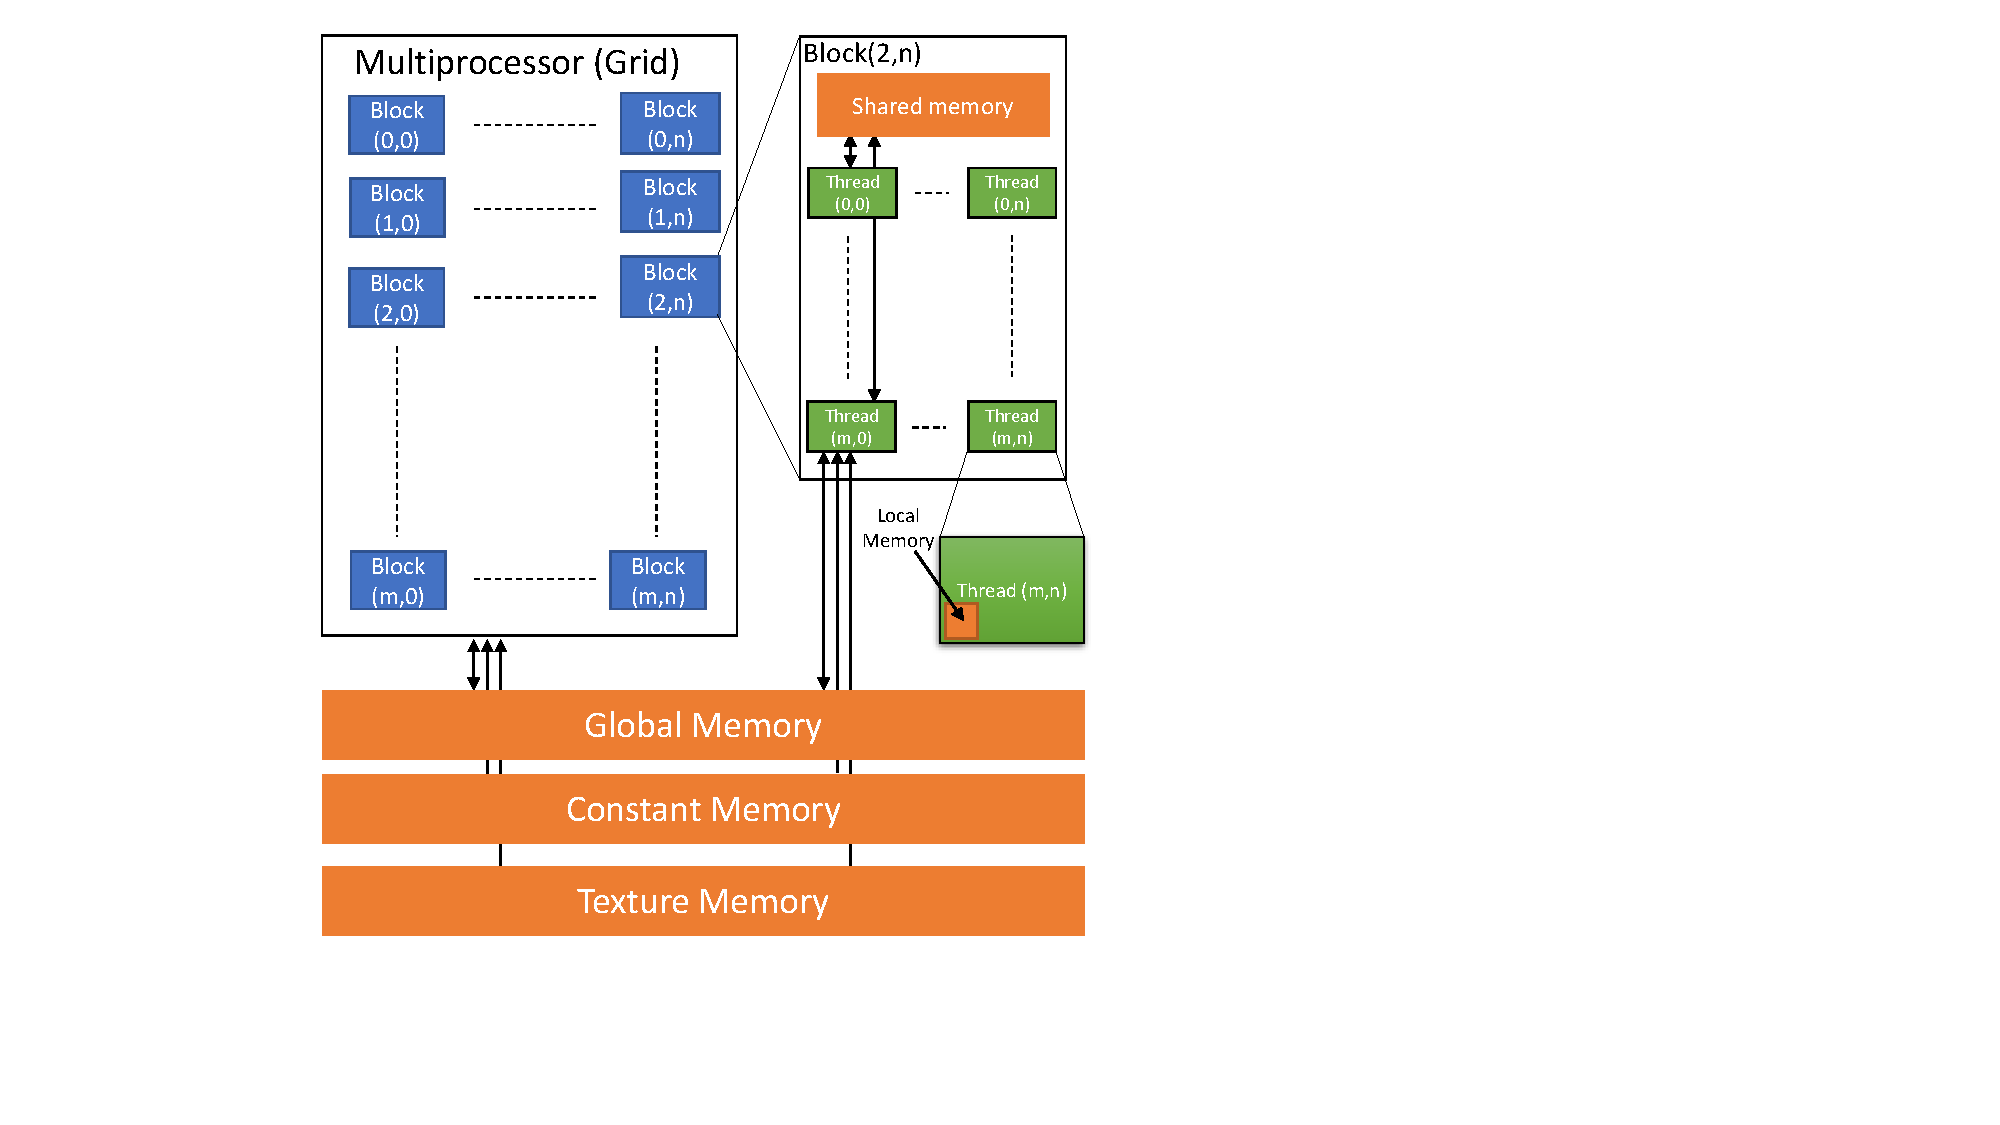
\includegraphics[scale=0.5]{Figure_1.pdf}
\caption{The parallel structure matrix inside the GPU and the various memories associated 
with each structure.}
\label{fig:bkg_gpu_arch}
\end{figure}


\subsection{Previous parallelized PBM works}
PBMs with large number of internal and external coordinates are computationally intensive. 
Thus, several researchers have made attempts to increase 
the speed of these simulations. \cite{Gunawan2008} developed a parallelization technique 
using a high-resolution finite volume solution of the PBM. The studies carried out by 
\cite{Gunawan2008} for their parallel PBM algorithm achieved good parallel efficiency upto 
100 cores. This study was limited by the number of grids used for the PBM,which meant the 
problem size was not computationally very heavy. This study also suggested that an algorithm 
with a shared memory model could help improve simulation speeds further. A hybrid memory model 
which uses both shared and local memory was implemented by \cite{Bettencourt2017} to 
obtain speed improvements of about 98\% from the serial code. This implementation took 
into account both Message Passing Interface (MPI) as well as Open Multi-processing (OMP). 
A similar PBM parallelization approach was also undertaken in \cite{Sampat2018} and an 
approximate speedup of 13 was obtained. The reduction in speed was attributed to the use of 
dynamic arrays used in their PBM framework to accommodate the hybrid nature of the model 
being used. 

Algorithms to parallelize the PBM codes on GPU have been studied briefly by Prakash et al.
\cite{Prakash2013b} using the inbuilt MATLAB's parallel computing toolbox (PCT).
\hl{They divided the operations of the nested loops into slices which would only use 240 cores of GPU.} 
This study was able to achieve good speedup values but could have been higher 
if the code had been implemented in native 
programming languages such as C or FORTRAN. Since MATLAB is a high level language it internally 
converts the written code to native programming languages before it is sent to the processor 
leading to excess computation which can be avoided \citep{pctMatlab}. Prakash et al. 
\cite{Prakash2013a} \hl{have shown that it is aggregation followed by breakage are responsible 
for the majority of the simulation time of the PBM due to the nested integrals in the formation 
and depletion terms. The continuous growth terms are not computationally intensive in 
comparison. Thus, the PBM in this work focuses on only discrete growth terms.} Other works that have 
used GPU acceleration to improve computation times for their population balance simulations 
include those from various other chemical engineering processes such as crystallization 
\citep{Szilagy2016}, combustion \citep{Shi2012} , multiphase flow \citep{santos2013}, 
coagulation dynamics \citep{Xu2015}. Several of these works fail to address the problem 
size as a factor in determining number of GPU cores used for the simulation. These algorithms 
are restricted to a maximum number of cores that are used and with an increase in the 
problem size, the algorithm would not adapt to increase the number of cores used. 
This could potentially lead to computation power that may go unused in high-end GPUs that 
have the capacity to perform several teraflops of double-precision calculations.


\section{Method and implementation}
\label{secMethods}
\subsection{PBM implementation}
The overall population balance equation with a lumped liquid and gas coordinates can be represented as:
\begin{align}
\frac{d}{dt}F(s_i,x,t)&=\Re_{agg}(s_i,x,t)+\Re_{break}(s_i,x,t)\notag\\ 
&+\dot{F}_{in}(s_i,x,t)-\dot{F}_{out}(s_i,x,t)
\label{eqn:mthds_pbm_overall} 
\end{align}
where, $F(s_i,x)$ represents the number of solid particles of type \textit{i} being studied in each spatial 
compartment $x$ of the granulator. The rate of aggregation $\Re_{agg}(s_i,x)$ 
and the rate of breakage $\Re_{break}(s_i,x)$ determines the rate at which particles density
changes within different size classes. The rate of particles entering, $\dot{F}_{in}(s_i,x)$ 
and exiting, $\dot{F}_{out}(s_i,x)$, the spatial compartment due to particle transfer also 
affects their number in each size class. The rate of change of internal liquid volume in each 
particle can be calculated as: 

\begin{align}
\frac{d}{dt}F(s_i,x)&l(s_i,x)= 
\Re_{liq,agg}(s_i,x)+\Re_{liq,break}(s_i,x)+\dot{F}_{in}(s_i,x)l_{in}(s_i,x)\notag\\
&-\dot{F}_{out}(s_i,x)l_{out}(s_i,x)+F(s_i,x)\dot{l}_{add}(s_i,x)
\label{eqn:mthds_pbm_rate} 
\end{align}
where, $l(s_i,x)$ is the internal liquid volume in each particle with ${s_i}$ as the 
solid volume for solid type \hl{\textit{i}} in the spatial compartment $x$. 
$\Re_{liq,agg}(s_i,x)$ and $\Re_{liq,break}(s_i,x)$ are the rates at which liquid is transferred 
between size classes due to aggregation and breakage respectively. $l_{in}(s_i,x)$ 
and $l_{out}(s_i,x)$ are the internal liquid volumes of the particles entering and exiting 
the spatial compartment. $\dot{l_{add}}(s_i,x)$ is the rate of volume of liquid acquired 
by each particle in the compartment at every time step due to external liquid addition.
Similarly, the rate of change of gas volume is calculated using the following equation: 

\begin{align}
\frac{d}{dt}F(s_i,x)g(s_i,x)&= 
\Re_{gas,agg}(s_i,x)+\Re_{gas,break}(s_i,x)+\dot{F}_{in}(s_i,x)g_{in}(s_i,x)\notag\\
&-\dot{F}_{out}(s_i,x)g_{out}(s_i,x)+F(s_i,x)\dot{g_{cons}}(s_i,x)
\label{eqn:mthds_pbm_gas_agg} 
\end{align}
where, $g(s_i,x)$ is the gas volume of each particle with solid volumes of $s_i$ 
in the spatial compartment $x$. $\Re_{gas,agg}(s_i,x)$ and $\Re_{gas,break}(s_i,x)$ are 
the rates of gas transferred between size classes due to aggregation and 
breakage respectively. 
$g_{in}(s_i,x)$ and $g_{out}(s_i,x)$ are the gas volume of the particles entering and 
leaving the spatial compartment respectively. $\dot{g_{cons}}(s_i,x)$ represents 
rate of the volume of 
gas particles formed due to process of consolidation occurring inside the system. The 
rate of aggregation, $\Re_{agg}(s_i,x)$ in Equation \ref{eqn:mthds_pbm_overall} is 
calculated as \citep{Chaturbedi2017}:

\begin{align}
\Re_{agg}(s_i,x)&= \frac{1}{2}\int _0^{s_i} \int _0^{s_i'} 
\beta(s_i',s_i-s_i',x)F(si',x)F(s_i-s_i',x)ds_ids_i'\notag\\ 
&- F(s_i,x)\int _0^{s_{max_i}-s_i} 
\beta(s_i,s_i',x)F(s_i',x)ds_i'
\label{eqn:mthds_R_agg}
\end{align}
where, $\beta(s_i, s_i',x)$ is the aggregation kernel and is expressed as a 
function of collision frequency ($C$) and collision efficiency ($\psi$). Further 
information on the model can be found in \ref{app:aggKernel}.

Similarly, the breakage rate can be expressed as follows:
\begin{align}
\Re_{break}(s_i,x)  = \int_0^{s_{max_i}} & \notag
K_{break}(s_1',s_2',x)F(s_1',s_2',x)ds_i' \\ &  - K_{break}(s_i,x)F(s_i,x)ds_i
\label{eqn:mthds_pbm_breakage_geneq}
\end{align}   
where, $K_{break}(s_i,x)$ is the breakage kernel. The formulation for the breakage 
kernel is discussed in more detail in \ref{app:breakKernel}.

The rate of increase of liquid volume of inside a particle, 
$\dot{l}_{add}(s_i,x)$ is expressed as:

\begin{align}
\dot{l}_{add}(s_i,x) = \frac{\sum_is_i\times\dot{m}_{spray}}{m_{solid}(x)}
\label{eqn:mthds_liq_addn_rate}
\end{align}
where, $\sum_i s_i$  is the total solid volume of the particle; $\dot{m}_{spray}$ is the 
rate of external liquid addition and $m_{solid}$ is the total amount of solid present in the compartment.

Particle transfer rate, $\dot{F}_{out}(s_i,x)$ in Equation \ref{eqn:mthds_pbm_overall} 
is calculated as:

\begin{align}
\dot{F}_{out}(s_i,x) = \dot{F}(s_i,x)\frac{\nu_{compartment}(x)\times dt}{d_{compartment}}
\label{eqn:mthds_f_out_dot_part_trans_rate}
\end{align}

where, $\nu_{compartment}(x)$ and $d_{compartment}$ are respectively the average 
velocity of particles in compartment $x$ and the distance between the mid-points 
of two adjacent compartment, which is the distance particles have to travel to 
move to the next spatial compartment. $dt$ is the time-step.

A finite difference method was used to solve the developed system of ordinary differential 
equations (ODEs) \citep{Barrasso2015cerd}. 
Euler integration was used as the numerical integration technique for its speed 
improvements and its minimal impact on accuracy \citep{Barrasso2013}.To avoid numerical 
instability due to the explicit nature of the Euler integration, Courant-Friedrichs-Lewis 
(CFL) condition must be satisfied~\citep{courant1967}. For our PBM model, time-step was 
calculated at each iteration such that, the number of particles leaving a particular bin 
at any time was less than the number of particles present at that time \citep{Ramachandran2010}.

\subsection{MPI implementation}
The message passing interface (MPI) parallel implementation of the PBM was 
focused towards equal distribution of the task and memory. The implementation 
used in this work differs from the hybrid implementation used by \citep{Bettencourt2017}
and \cite{Sampat2018} as only MPI was used to parallelize the code. It 
was pointed by \cite{Sampat2018} that open multi-processing(OMP) does not 
provide significant speed improvements due to limitations with usage of 
dynamic vectors which are essential for such a system. Thus, the OMP 
implementation was avoided which also meant that lesser number of cores 
would be required. The focus of this study to localize the computation power 
rather than depend on supercomputers/clusters.  
A pseudo code has been presented in Algorithm \ref{alg:CPUparallelPBM}
to illustrate the distribution of tasks. For each time step, a MPI process is responsible 
for a certain section of the problem, usually a spatial chunk inside the geometry 
(also referred to as compartment).  



Simulations for this study were performed on a computer with an Intel Core i7-7700K 
processor clocked at 4.2GHz and 32 GB of RAM. For maximum performance while 
data reading and writing a SSD was used. GCC version 7.4 with openMPI 2.0 
was used to compile the parallel C++ code.

\begin{algorithm}
     \scriptsize
     \caption{CPU-based Parallel Population Balance Model}
     \label{alg:CPUparallelPBM}
     \begin{algorithmic}[1]
     \Procedure{PBM}{$N_{Comp}$,$N_{MPI}$}\Comment{$N_{Comp}$ is the number of compartments}
     \State \texttt{Divide $N_{Comp}$ in $N_{MPI}$}
     \While{$t < t_{final}$}
     \For{$\forall n_{Comp}$ in 1 MPI process}
     \State \texttt{Calculate $\Re_{aggregation}$ for solid bins $s_1$,$s_2$}
     \State \texttt{Calculate $\Re_{breakage}$ for solid bins $s_1$,$s_2$}
     \State \texttt{Calculate $n_{particles}$ using Euler's method}
     \EndFor
     \State \texttt{Collect $n_{particles}$ from $N_{MPI}$}\Comment{Master process collects all data}
     \State \texttt{Calculate $timestep$ using \textit{CFL} condition}
     \State \texttt{$t_{new} = t + timestep$}
     \EndWhile
     \EndProcedure
     \end{algorithmic}
 \end{algorithm}   


\subsection{GPU implementation}
NVIDIA\textsuperscript{\tiny\textregistered}’s CUDA\textsuperscript{\tiny\textregistered} 
toolkit extends the C language such that user defined functions 
called kernels can be created to be run on the GPU. These kernels can be 
executed several number of times in parallel using large number of threads. 
A thread is a sequence of programmed instructions that can be managed by the 
computer’s scheduler. A kernel depending upon the dimensions of the data can execute 
instructions in 1-D, 2-D or 3-D thread blocks. The kernel can also launch 
multiple thread blocks at once, thus increasing the number of parallel 
process executions known as grid. Similar to a thread block, a grid can 
range from 1-D to 3-D depending upon the data under study.
The code execution was split between the CPU (also called host) and GPU 
(also called device). Time sensitive calculations and calculations that
require collection of data from the GPU were handled on the CPU 
using a single core, while the more computationally intensive tasks were distributed 
on to the GPU using kernels. Similar to the parallelization using MPI in CPUs, the 
geometry was split into multiple compartments. \hl{These compartments determined the number of 
blocks inside each GPU kernel. The number of solids used helped formed 
the threads in each of these blocks.} The work flow of the execution can 
be found in Figure \ref{fig:mtd_gpu_imp}. The arrows in Figure \ref{fig:mtd_gpu_imp} 
indicate the interchange of data between the CPU memory to the GPU memory. 




\begin{algorithm}
     \scriptsize
     \caption{GPU-based Parallel Population Balance Model}
     \label{alg:GPUparallelPBM}
     \begin{algorithmic}[1]
     \Procedure{PBM}{$N_{Comp}$}\Comment{$N_{Comp}$ is the number of compartments}
     \State\texttt{Copy initial variables from CPU memory to GPU memory}
     \State \texttt{GPU initial calculation kernel call from CPU}\Comment{Performed on GPU}
     \State \texttt{Divide $N_{Comp}$ in $N_{blocks}$}
     \State \texttt{Copy back initial values to the CPU RAM}
     \While{$t < t_{final}$}
	 \State \texttt{Copy time-dependent process variables from CPU to GPU RAM}
     \State \texttt{GPU aggregation rate kernel call from CPU}
     \State \texttt{Calculate $\Re_{agg}$ for solid bins $s_1$,$s_2$}\Comment{Performed on GPU}
	 \State \texttt{GPU aggregation rate kernel call from CPU}     
     \State \texttt{Calculate $\Re_{breakage}$ for solid bins $s_1$,$s_2$}\Comment{Performed on GPU}
     \State \texttt{Calculate $n_{particles}$ using Euler's method}
     \State \texttt{Copy back process rate data back to the CPU RAM}
     \State \texttt{Calculate $timestep$ using \textit{CFL} condition}\Comment{Performed on CPU}
     \State \texttt{$t_{new} = t + timestep$ }
     \EndWhile
     \State \texttt{Clear GPU memory}
     \EndProcedure
     \end{algorithmic}
 \end{algorithm}

\newpage
\begin{figure}[th]
\centering
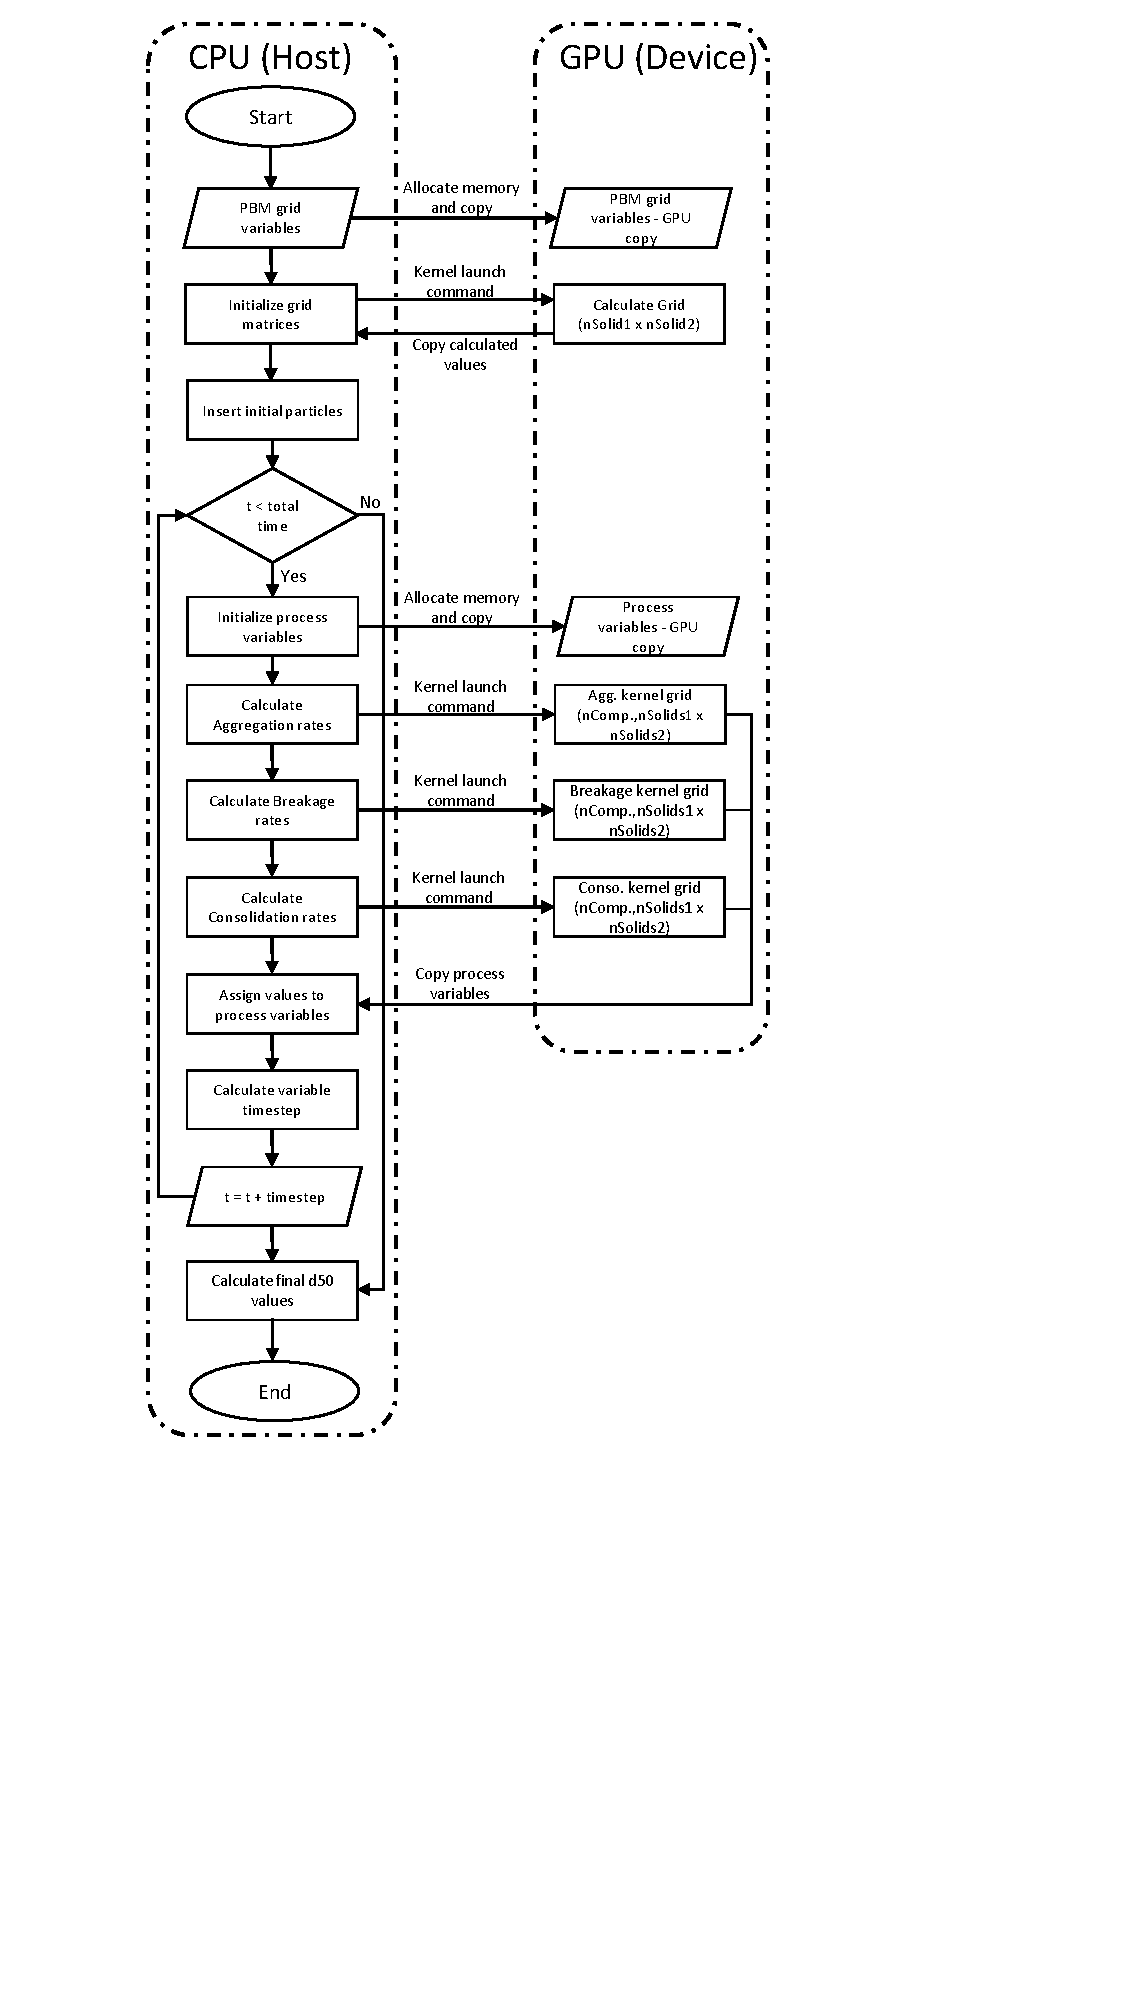
\includegraphics[scale=0.8,trim=200 250 300 200]{Figure_2.pdf}
\caption{Workflow of the GPU code indicating data transfers and execution timeline of the code.}
\label{fig:mtd_gpu_imp}
\end{figure}


\newpage
\section{Results and discussions}
\label{secResults}
 \subsection{Performance metrics}
Parallel efficiency of an algorithm can be tested either by strong scaling, 
where the problem size remains the same and number of processing elements 
are increased or by weak scaling, where the number of processing elements 
remain the same and the problem size is increased. In this study, the 
number of processing units were limited due to the architecture of the 
GPU and the CUDA\textsuperscript{\tiny\textregistered} C++ code developed did not utilize more than one GPU 
during execution. Thus, a weak scaling approach was preferred in such a 
scenario. The parallel performance of a code is usually measured in 
terms of on ratio of time taken to solve the run the simulations on one 
core to the time taken to run the simulation on N cores. It is depicted in
Equation \ref{eqn:result_parallelefficiencyWeak}, where $t_1$ is the time taken 
to the run the problem on one core where as $t_N$ is the time taken to 
run the problem on N cores.

\begin{align}
\ Speedup = \frac{t_1}{t_N}
\label{eqn:result_parallelefficiencyWeak}
\end{align}

The problem size was varied by increasing the number of compartments inside 
the PBM. This in turn increased the total number of calculations performed 
without increasing the amount of work that needed to be performed by each 
processing unit (core). The number of cores required during the simulation 
on the GPU was determined by the product of the number of compartments and 
the number of solid bins for each solid type used. Thus, the number of GPU 
cores used in this study varied from 256 cores for 1 compartment to 8192 
for 32 compartments.

Parallelization of code can lead to deviation in calculations from 
the serial execution. This discrepancy in calculation can be attributed to 
the difference in the precision of the cores of the CPU or GPU being used. 
This change in precision can lead to a small error in one timestep, which can 
percolate and produce results that can drastically different from the serial 
code. To check the validity of the presented algorithm a relative least sum 
of squares error was calculated as shown in Equation \ref{eqn:result_rSSe}:

\begin{align}
rSSE =  \sum_{i=0}^{t_{end}} \frac{(d_{50_{serial_i}}-d_{50_{parallel_i}})^2}{N}
\label{eqn:result_rSSe}
\end{align}

The $rSSE$ was calculated for the algorithm considering the single core MPI 
solution as the base and determining the error values \hl{with respect to} to this simulation.
The error for each of the case can be found in Figure \ref{fig:res_gpu_error}. The error 
for the GPU simulations varied from $0.45\%$ to about $6\%$ which is an acceptable 
range. Thus, making the solutions from the algorithm quicker with a very small 
loss in accuracy. There was an increase in the error with the increase in number 
of compartments, which could be due to the increase in the number of data points compared. 

\begin{figure}[H]
\centering
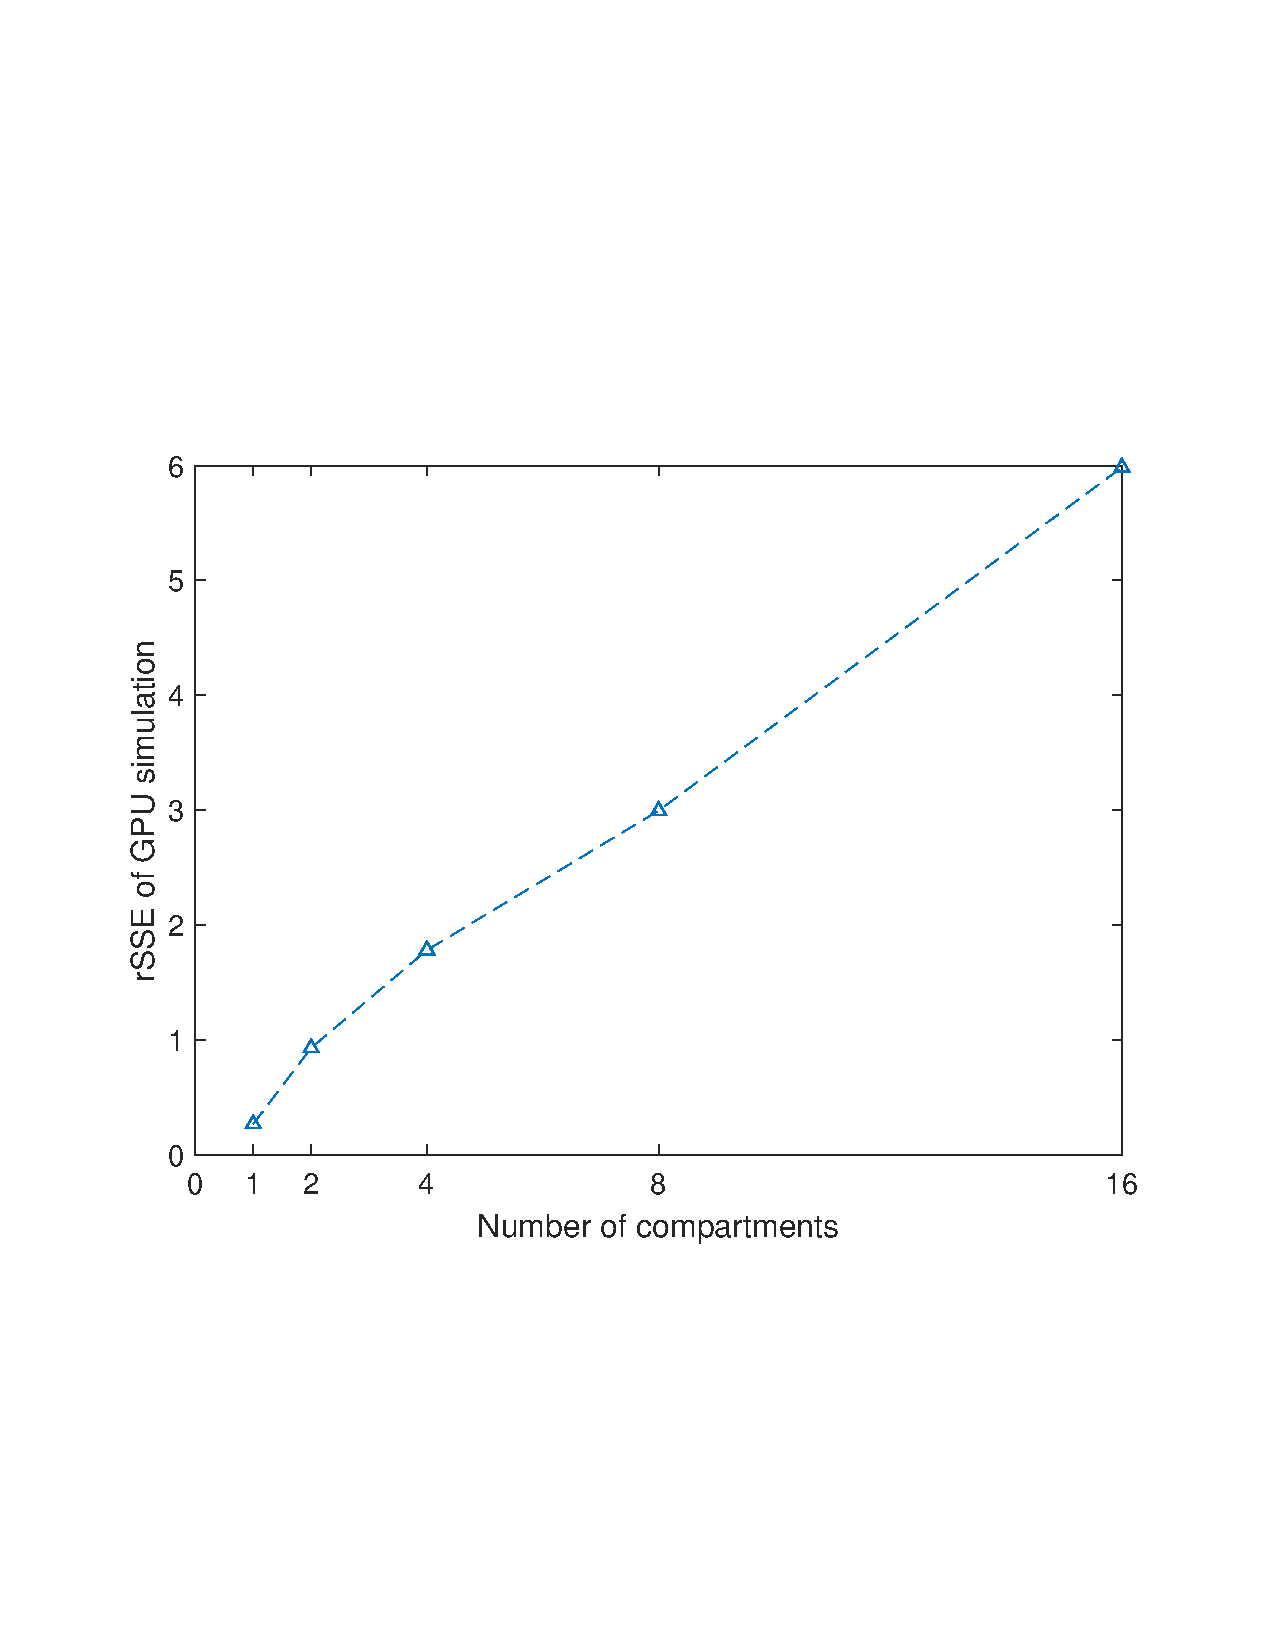
\includegraphics[scale=0.7,trim=50 180 50 200, clip]{Figure_3.pdf}
\caption{Relative sum of square error observed for the GPU simulations compared to 
the serial simulation}
\label{fig:res_gpu_error}
\end{figure}


\subsection{Algorithm performance on a desktop GPU}
The desktop configuration used for these studies comprised of a Intel $i7-7700K$  
CPU clocked at $4.5$ GHz with $32$ GB DDR4 RAM and a 
NVIDIA\textsuperscript{\tiny\textregistered} Quadro $P4000$ GPU. 
The NVIDIA\textsuperscript{\tiny\textregistered} Quadro GPU used had 1792 
CUDA\textsuperscript{\tiny\textregistered} cores with 8 GB of GDDR5 RAM. 
CUDA\textsuperscript{\tiny\textregistered} version 9.0 paired with GCC 7.3 was 
used to the run the desktop GPU simulations with Ubuntu 18.04 operating system (OS).

The number of solid bins for the 2 different types of solids used were $16$, 
this meant that there was a maximum of $65,536$ calculations that needed to 
be performed for each time step for each compartment. While, the
number of calculations increased to over 2 million per time step when the number of 
compartments was increased to $32$. Each GPU consisted of several streaming 
multi-processors(SM) which help distribute the problem to the 1792 cores inside 
the GPU. Once the calculations  pass from the CPU to the GPU, the SMs take 
over and allocate work to the GPU in blocks of $32$ threads each. 
SMs divide these calculations in blocks 
of 32 threads and send it to the cores for calculations which accounts for some 
overheard time during the simulation. This overhead is present for each timestep, 
which can be compensated by the number of calculations running in parallel on 
the GPU. 

The PBM simulation was run for $90$ seconds which included $45$ seconds of mixing 
and 45 seconds of liquid addition. The algorithm performance was tested by weak scaling 
the problem by changing the number of compartments from $1$ and doubling them in 
each simulation until the number of compartments reached $32$. Figure \ref{fig:res_gpu_timings} 
shows the time taken these simulation. It can be observed that the amount of time taken 
for the simulation remains almost constant till the number of compartments reaches $8$, 
followed by an increase in the time taken as the number of compartment are increased 
further to $32$. According to parallelization procedure used the cores utilized to run the 
code is directly proportional to the number of compartments and the number of solid bins 
present in the problem. The constant time is a result of the problem size being smaller than 
the Quadro $P4000$'s 1792 CUDA\textsuperscript{\tiny\textregistered} core, i.e. 
the algorithm was not able to utilize all the 
CUDA\textsuperscript{\tiny\textregistered} cores till the compartment number was $8$. 
Since the algorithm uses about $256$ cores 
to simulate each compartment, the cores would not suffice once the compartment number reaches 
$16$ and the SMs would have to wait to distribute the calculation to cores once 
initially allocated calculations are finished. This wait time leads to the increase in the 
time of simulations as seen in the case for $16$ and $32$ compartments. 

\begin{figure}[H]
\centering
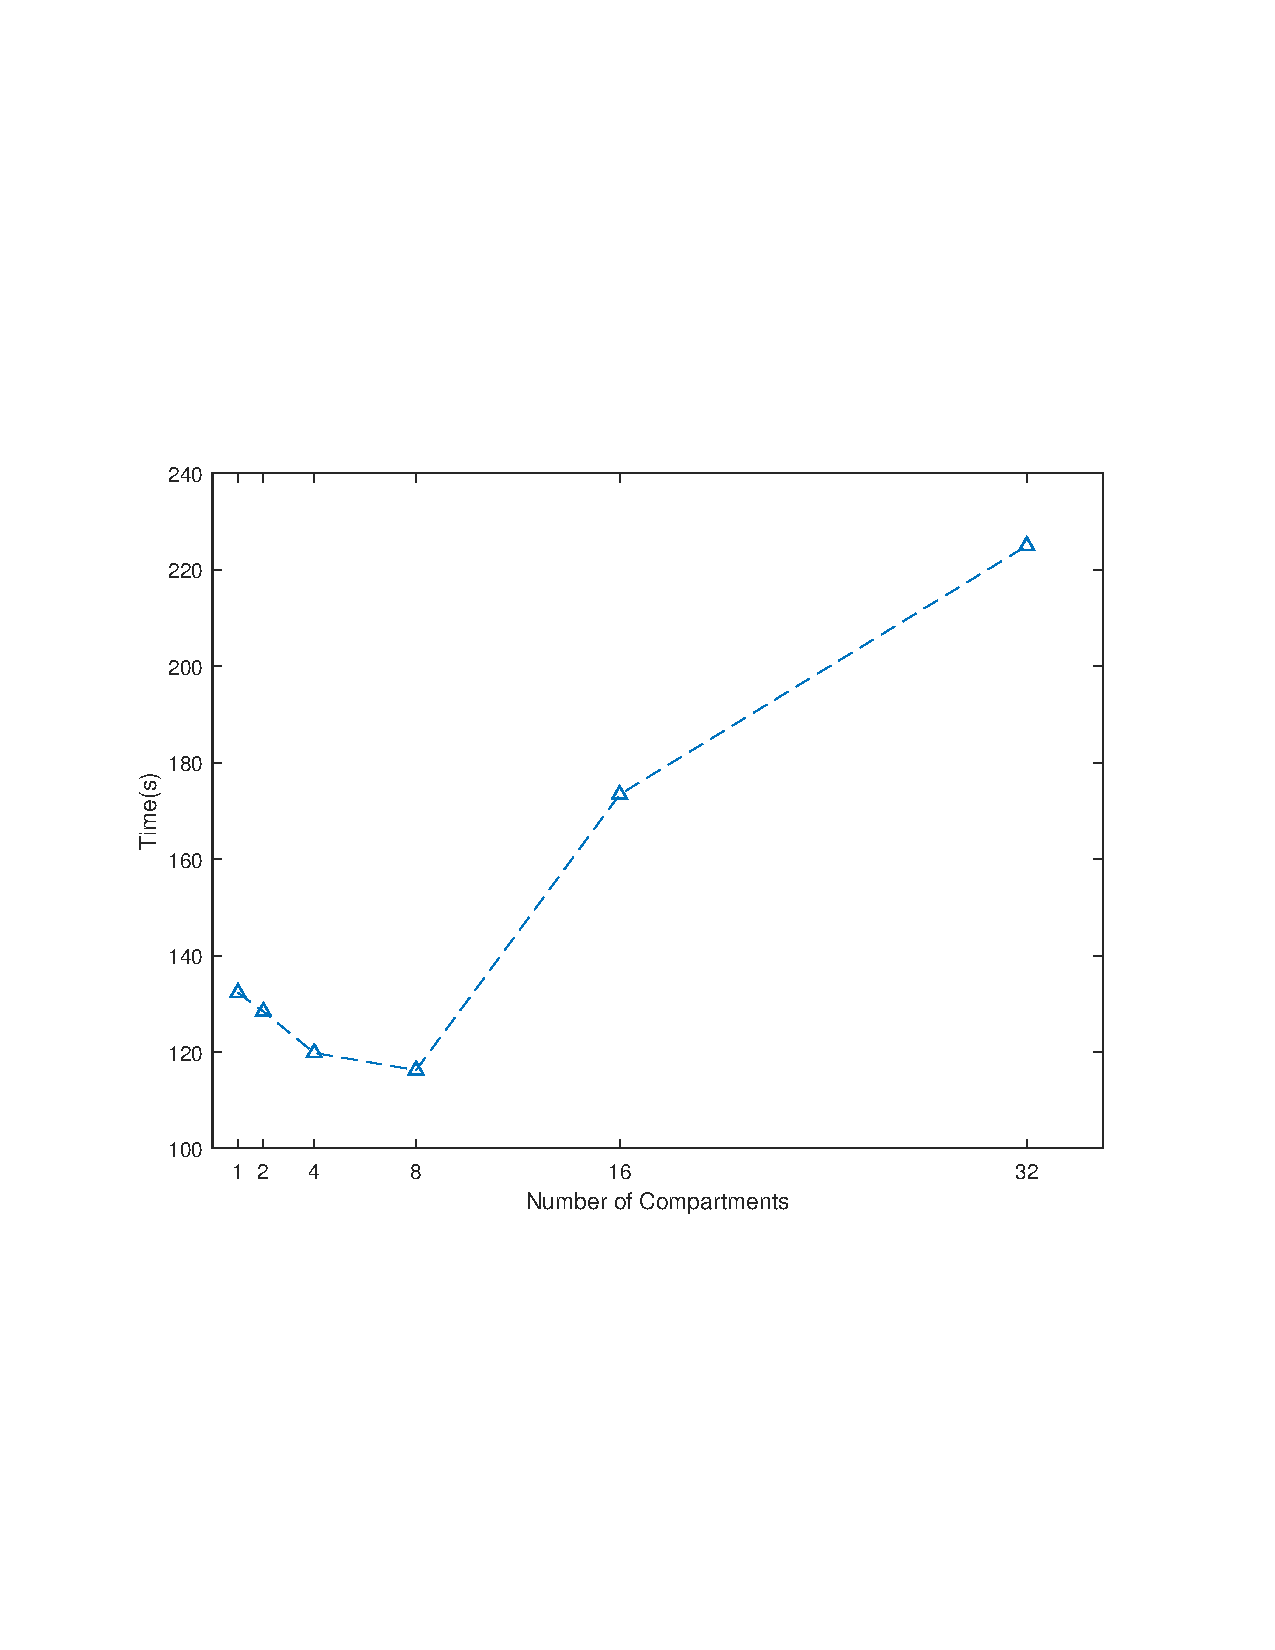
\includegraphics[scale=0.7,trim=50 180 50 180, clip]{Figure_4.pdf}
\caption{Time taken to complete 90 seconds of PBM simulation with varying number of compartments 
on NVIDIA\textsuperscript{\tiny\textregistered} Quadro P4000 GPU}
\label{fig:res_gpu_timings}
\end{figure}


The above argument was supported by the profile of the code that was obtained using NVIDIA\textsuperscript{\tiny\textregistered}'s
inbuilt code profiler $nvprof$. Code profiling is an important step in algorithm development. 
The profiler results can be varied based on the options chosen to obtain the parameters being 
studied. In this case, API calls and GPU activity were exported to understand the performance 
bottlenecks and those sections of the code were rectified to improve the speed of the algorithm.
The profiler was executed for each case and it was observed that aggregation kernel calculations 
took the most time for execution followed by the breakage kernel. Consolidation kernel 
and other calculations comprised of less than $1$\% of execution time. The other parameter 
studied was the number of times each API was called by the code and the time spent. API 
calls included the synchronization of threads working inside the GPU device, memory allocation 
for arrays, etc. Each thread inside the GPU operates independently,
thus all threads may not be at the same section of the code at a given moment of time, 
thus some threads may finish calculations before others. The time taken to synchronize 
these threads required the most amount of time during the execution of the code. When 
such an API is called by the code further execution of the code is paused until all 
the threads of the GPU are in the same line of code. This accounted for $99\%$ of the total  
other API call time. This indicated that there were not many places where the code could 
have been optimized further since synchronization statements were only added before 
calculations where complete array of data was required. 
If further reduction in these statements was undertaken, it would lead to data loss and 
possibly incorrect final calculated particle size distribution. A comparison of times taken 
by each process in the simulations is shown in Figure \ref{fig:res_profile_pie}. A similar 
distribution of times was observed for all simulations on the GPU.

\begin{figure}[H]
\centering
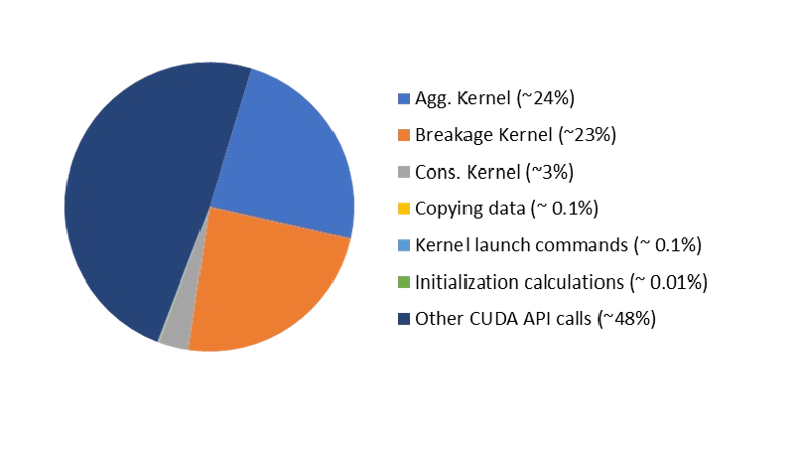
\includegraphics[scale=1]{Figure_5.pdf}
\caption{Distribution of times taken by different processes inside the GPU-parallelized 
PBM}
\label{fig:res_profile_pie}
\end{figure}


\subsection{Performance on GPUs compared to CPUs}
The NVIDIA\textsuperscript{\tiny\textregistered} Quadro P4000 GPU used 
had its cores at a base clock speed of $1202$ MHz while
the CPU cores had a base clock of $4000$ MHz. The algorithm used to parallelize on the GPU 
did not permit the use of only one core of the GPU for simulation. Thus, a single MPI core 
CPU simulation was used as the baseline for all comparisons. Theoretically, it would take 
longer on a single core of the GPU to run a similar simulation than on a single GPU core

The CPU version of the parallel PBM was run on the desktop with the aforementioned 
configuration. This meant that the number of MPI cores available for the simulations 
was limited to 4. Weak scaling of the problem by changing the number of compartments 
was performed for this study. Figure \ref{fig:res_cpu_timings} shows a comparison of the times taken 
by the simulation to run on $1$, $2$ \& $4$ MPI cores. The times indicate that 
with the increase in the number of cores the model took less time to complete 
calculations for the same number of compartments. It can also be seen that for the 
same number of MPI cores used in a soft scaling the amount of time increases 
with increase in the number of cores. This increase can be attributed to the 
increase in the number of calculations with addition of new compartments. There is a 
plateau in the times when 2 and 4 MPI cores were used for $8$ and $16$ compartments 
respectively. When a further analysis of the rates was for each compartment was undertaken 
it was observed that till the particles did not each the last few compartments of the 
granulator no aggregation or breakage occurred in those spatial sections thus reducing 
the compute time and leading to similar simulation times.

\begin{figure}[H]
\centering
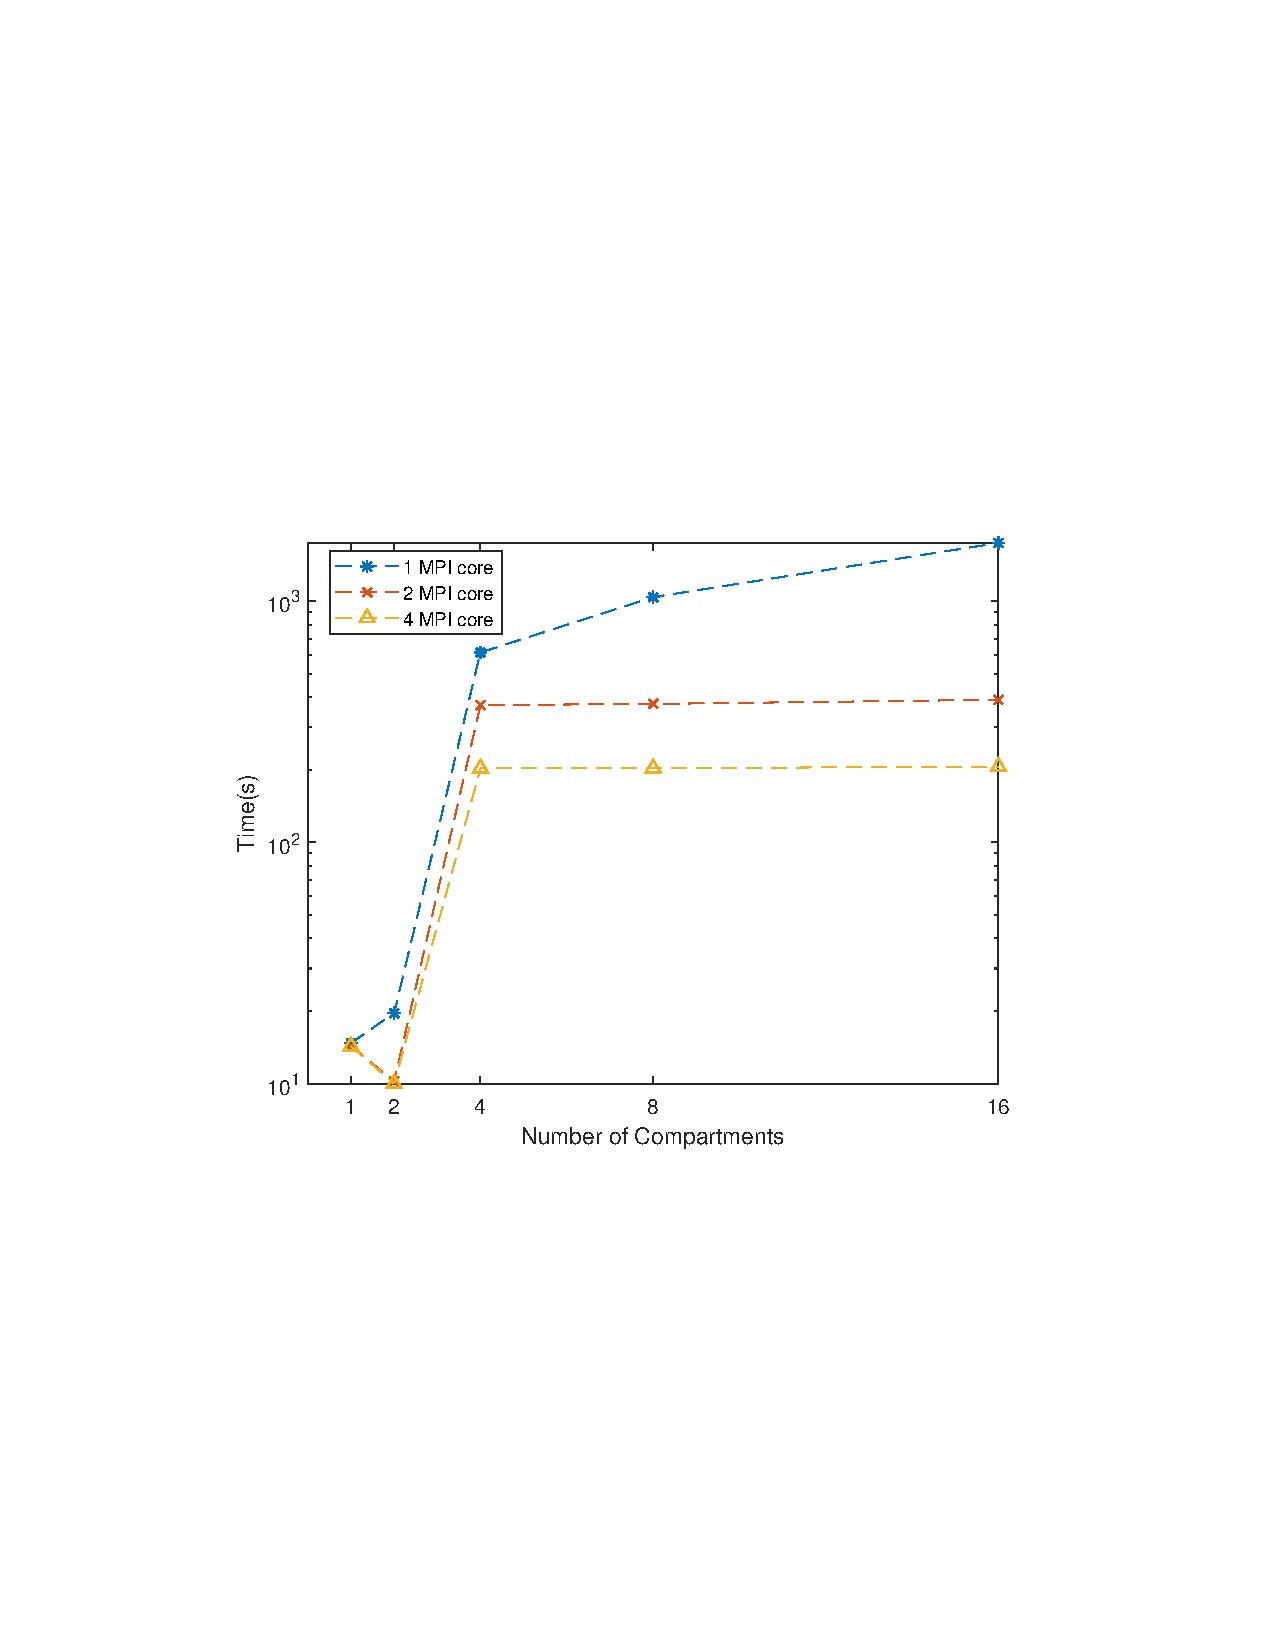
\includegraphics[scale=0.7,trim=100 240 100 240, clip]{Figure_6.pdf}
\caption{Time taken to complete 90 seconds of PBM simulation with varying number of compartments 
on desktop CPU with varying number of MPI cores}
\label{fig:res_cpu_timings}
\end{figure}

Speedup is important to understand the scalability and 
parallel performance of a code. Speedup for a code is directly proportional 
to the number of cores used for a simulation. 
In Figure \ref{fig:res_desktop_speedup}, the speedup increases with the increase in 
the number of MPI cores. This increase in speedup can be attributed to the increase 
in the computation power. 
One unusual trend observed in the case of 8, 16 and 32 number of compartments for both 
2 MPI and 4 MPI core simulations, the speedup is higher than 2 and 4 respectively. 
This phenomena is known as super linear speedup which occurs 
when the speedup is greater than the number of cores used. In rare cases like these
speedup increases due to increase in cache memory and random access memory(RAM) 
available \citep{tuncer2009}. The simulations with the GPU parallel code showed an 
overall increase in the speedup as the number of compartments as seen in Figure 
\ref{fig:res_desktop_speedup}. The speedup was low for compartment numbers 1 and 2 
since the amount of time spent in communication in between the CPU and the GPU as well 
as the time taken by the thread synchronization in the GPU to had a larger 
contribution to the simulation time. The increase in number of compartments diminished 
this communication time effect as amount of calculations is significantly higher. The 
highest speeedup achieved for a GPU simulation was about $12.3$, which means it took 
$12$ times less time than a serial CPU computation. 


\begin{figure}[H]
\centering
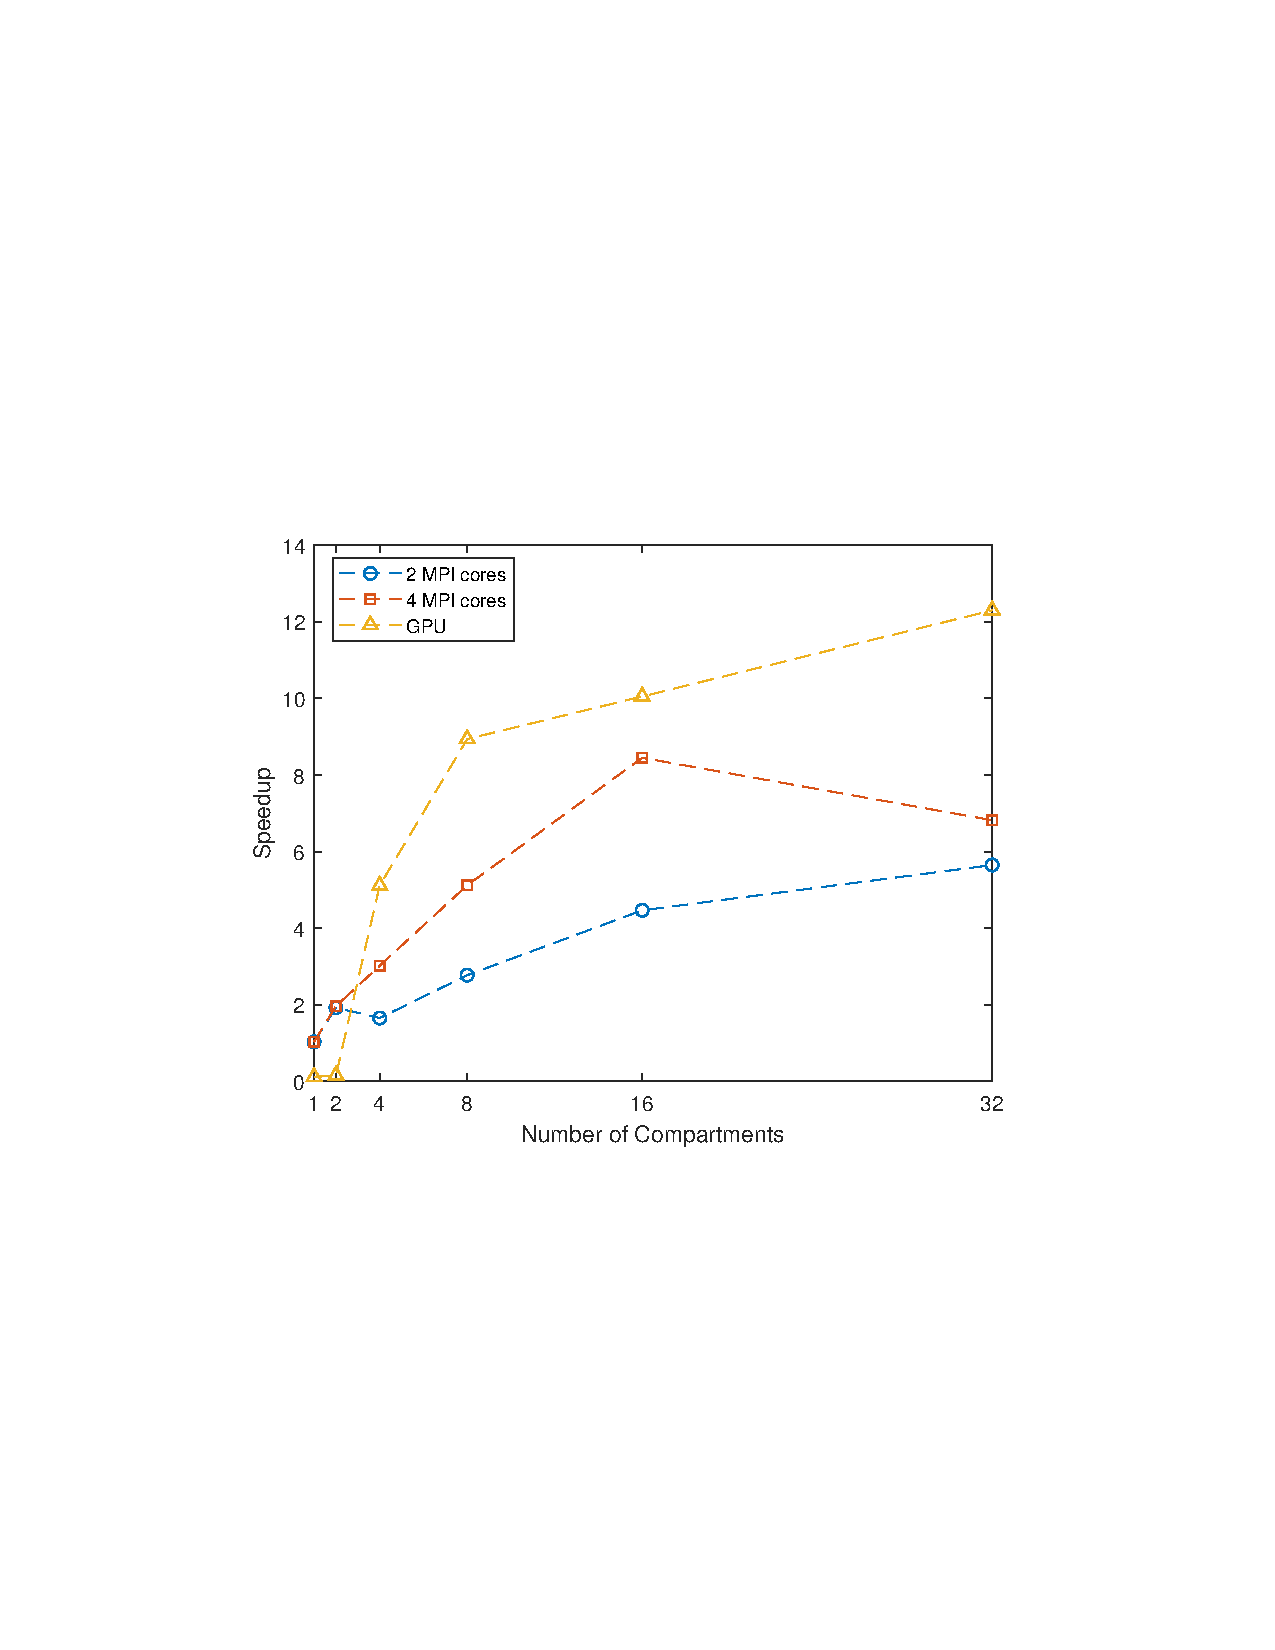
\includegraphics[scale=0.7,trim=120 240 120 240, clip]{Figure_7.pdf}
\caption{Comparing speedup for CPU and GPU simulations to respective serial simulations}
\label{fig:res_desktop_speedup}
\end{figure}



\subsection{Server level GPU code performance}
The high performance computing (HPC) device used to run the parallel PBM GPU code 
was present at Rutgers at the School of Engineering (SoE). The SoE HPC cluster was 
equipped with a NVIDIA\textsuperscript{\tiny\textregistered} Kepler K20 GPU. This GPU contains 2496 CUDA\textsuperscript{\tiny\textregistered} cores which are 
have a base clock of $706$ MHz and only 5 GB of GDDR5 of memory. The Kepler series 
GPUs were a couple of generations older than the Pascal generation Quadro P400 used 
in desktop simulation studies. The clock speed and memory of the desktop GPU were 
higher than the one present on the HPC. 

Time taken to complete the $90$ second PBM simulation on the HPC's GPU are shown in 
Figure \ref{fig:res_serverTimes}. The time taken to run the PBM initially remains 
constant upto 16 compartments, but a large increase in the time is observed for the 
simulation with 32 compartments. This increase could be attributed to the saturation 
of CUDA\textsuperscript{\tiny\textregistered} cores of the GPU and that SMs had to wait for the previous calculations to 
complete before the threads were assigned the remnant of calculations. This trend 
is similar to the trend observed in Figure \ref{fig:res_desktop_speedup} for the 
desktop GPU. A serial simulation was performed on the HPC and used as a baseline 
for speedup calculations. Speedup from the server GPUs are shown in Figure 
\ref{fig:res_serverSpeedup}. The increase in the speed of the simulation for these 
studies is lower than the desktop studies which could be directly connected to clock 
speeds of the CUDA\textsuperscript{\tiny\textregistered} cores. The server GPU cores were clocked at a lower frequency 
which meant the rate of calculations would decrease. One other reason for reduced 
speedup could be the older architecture of Kepler GPU which are slower in floating 
point calculations \citep{Pascal2016}.

\begin{figure}[H]
     \centering
     \begin{subfigure}[b]{0.48\linewidth}
         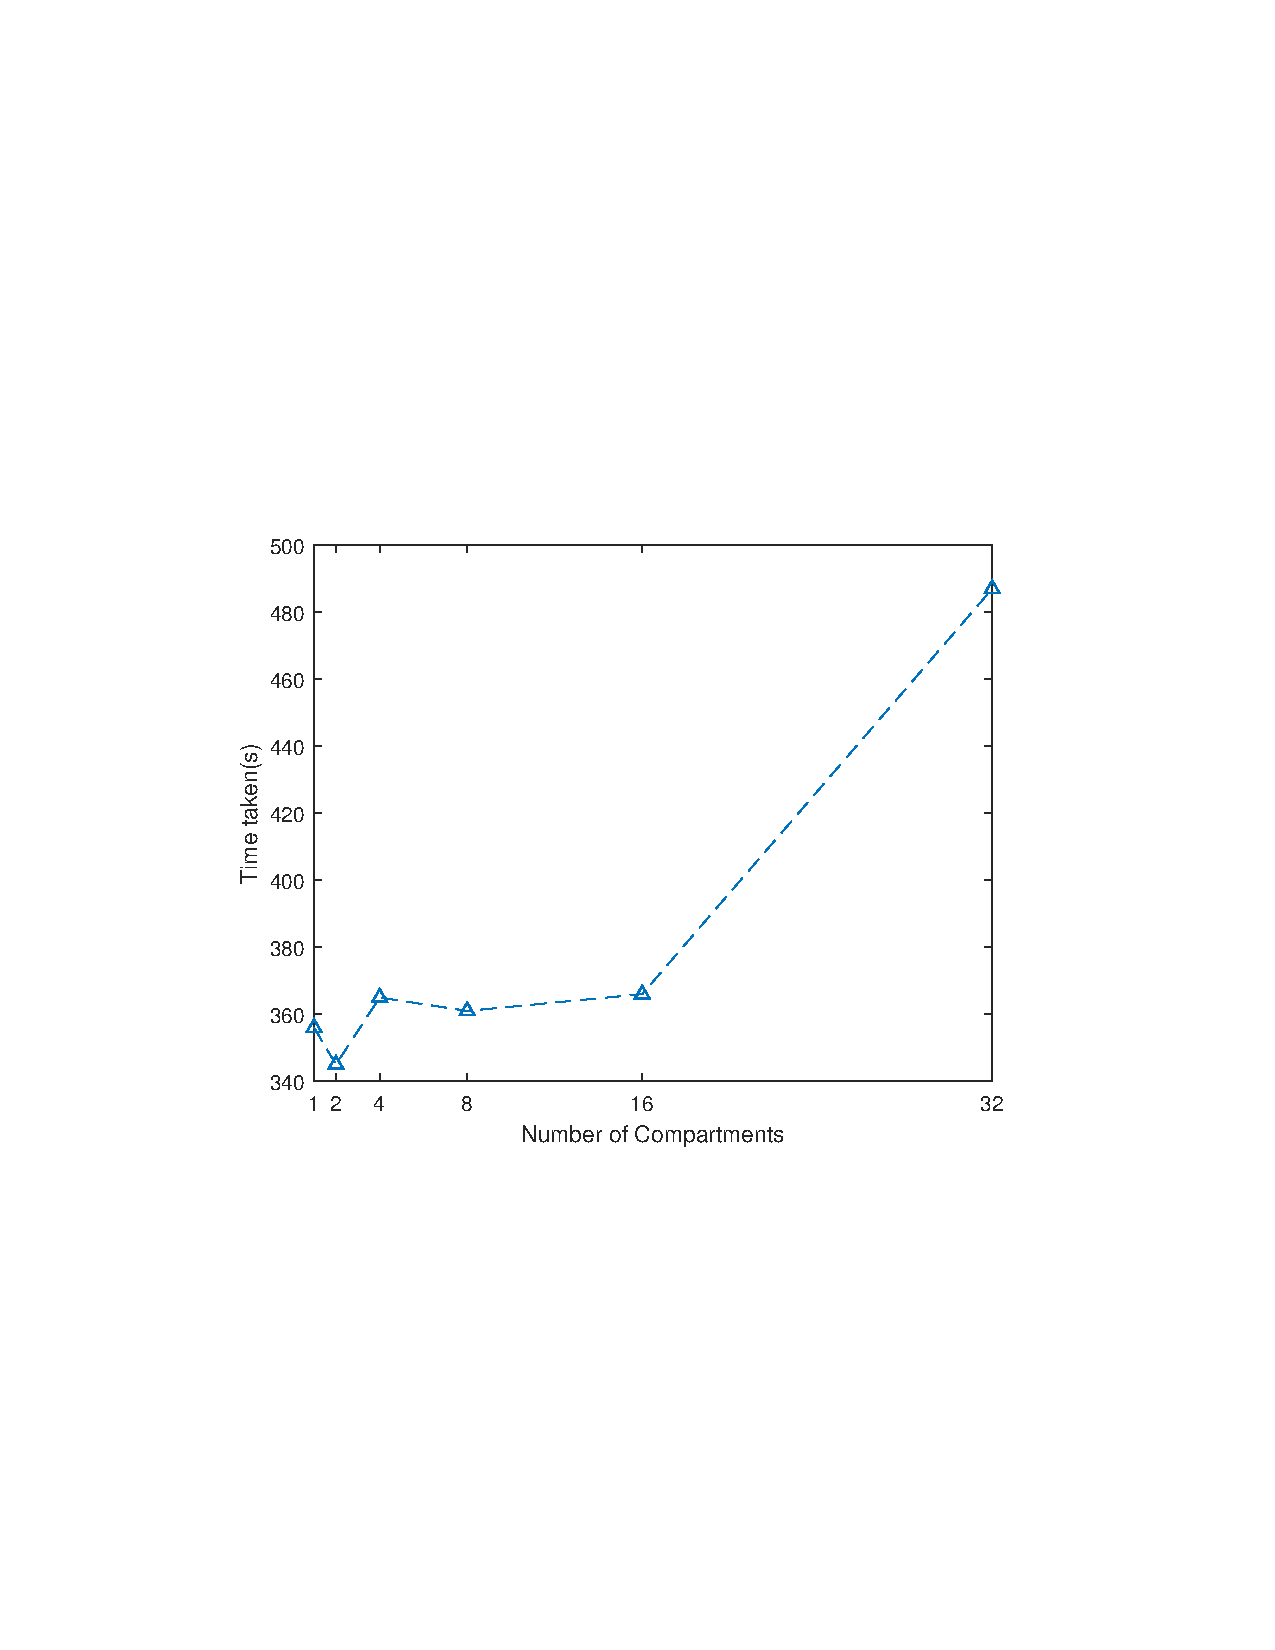
\includegraphics[scale=0.7,trim=120 240 120 240,width=\linewidth]{Figure_8a.pdf}
         \caption{}
         \label{fig:res_serverTimes}
     \end{subfigure}
     \hfill
     \begin{subfigure}[b]{0.48\linewidth}
         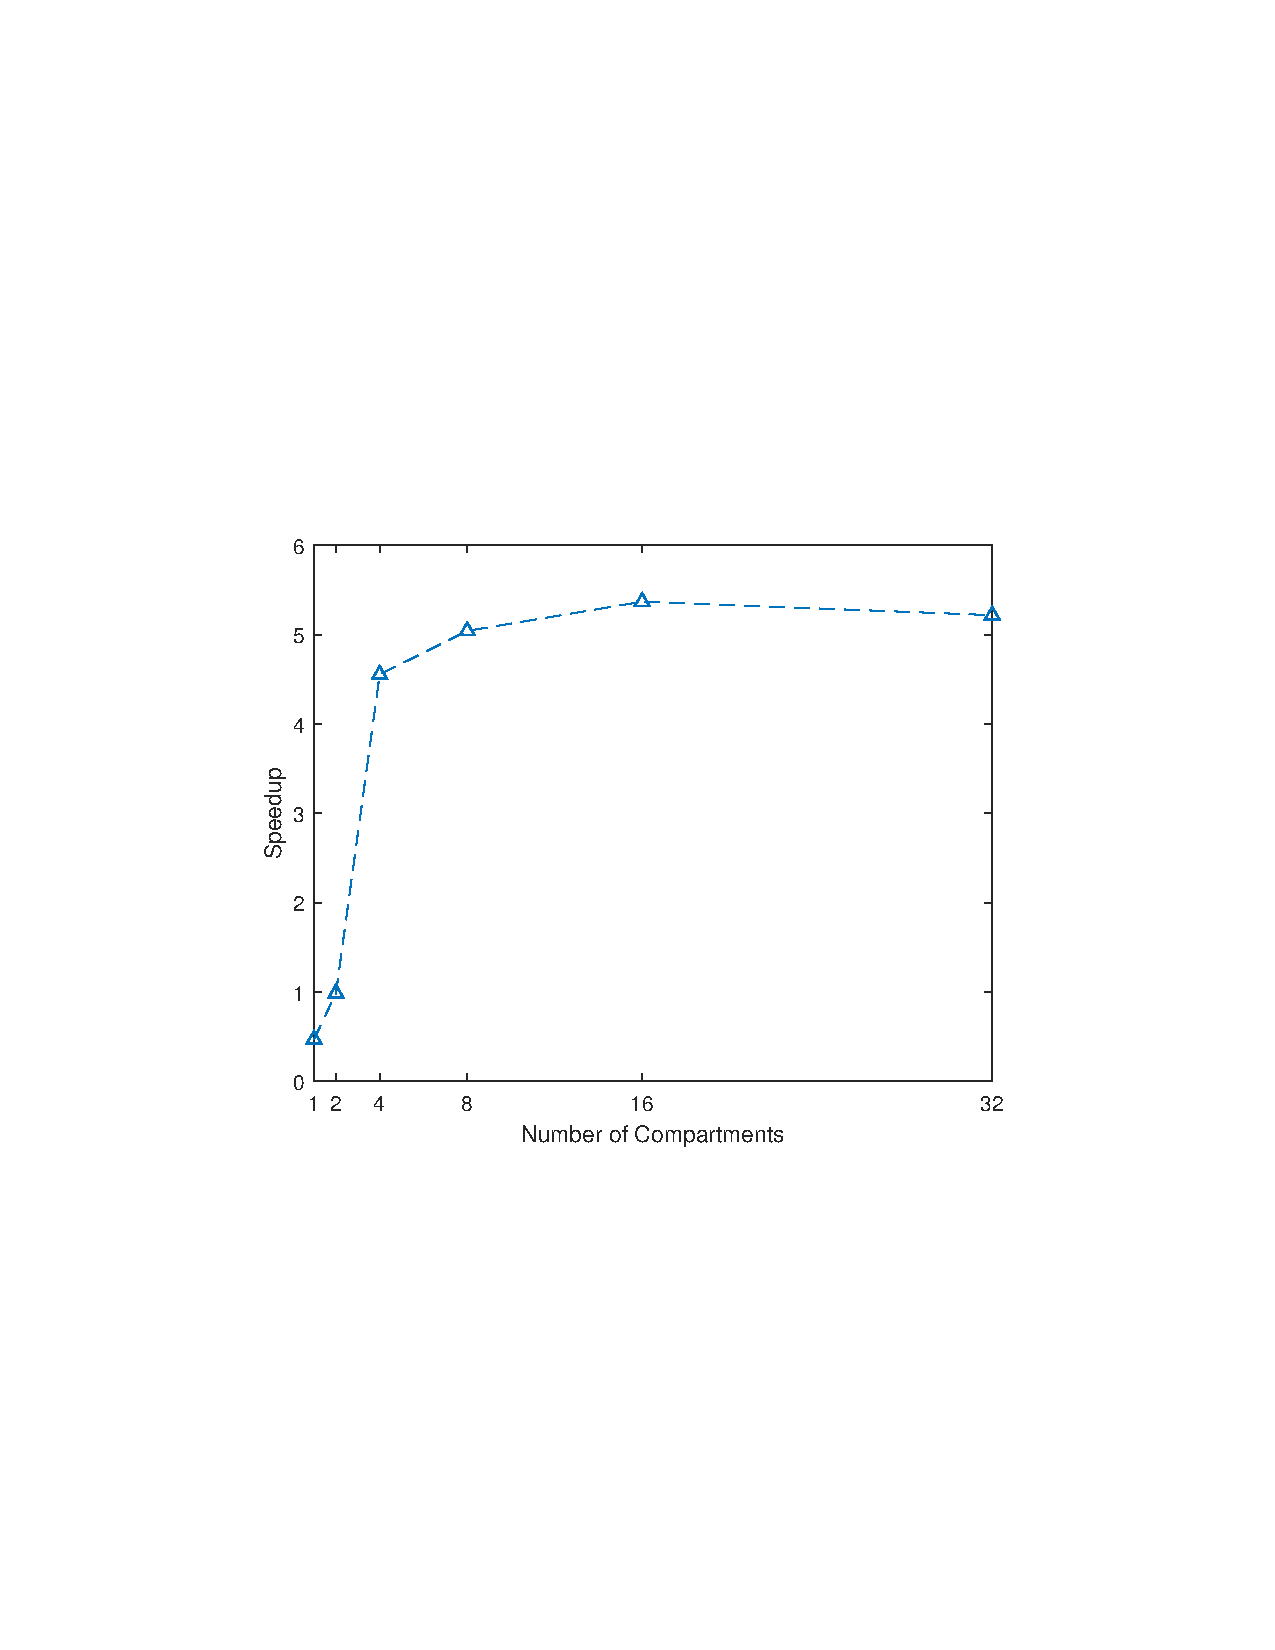
\includegraphics[scale=0.7,trim=120 240 120 240,width=\linewidth]{Figure_8b.pdf}
         \caption{}
         \label{fig:res_serverSpeedup}
     \end{subfigure}
        \caption{(a)Time taken to run 90s PBM simulation on HPC's Kepler K20 GPU 
        (b)Speedup achieved for the GPU simulation over the serial simulation on the HPC device}
        \label{fig:res_server}
\end{figure}



\section{Conclusions}
\label{secConc}
In the presented study, a PBM was developed using NVIDIA\textsuperscript{\tiny\textregistered}'s  CUDA\textsuperscript{\tiny\textregistered} C/C++ language 
to run in parallel on a GPU. The time of the simulations on the GPU were compared 
to CPUs. In cases with larger problem size, it was observed that GPU simulations 
were faster than CPU simulations and there was minimal loss in accuracy. 
It can be observed that GPUs are more efficient when the complexity of the 
problem is high in terms of compartments, which is a commonly observed in general 
application of PBMs. The adaptive structure of the algorithm 
enabled the simulation to use varying number of GPU cores to parallelize the PBM simulations.
The GPU architecture also plays a major role in the simulation time. This work also 
highlighted that a desktop PC could be sufficient for a computationally intensive 
simulation instead of a utilizing a supercomputer or cluster. \hl{A similar parallel strategy could  
be developed for growth terms for internal coordinates and other rate processes inside the PBM 
using CUDA kernels.} This work can be extended in the future by testing it on newer 
GPUs from NVIDIA\textsuperscript{\tiny\textregistered} 
like the Volta and Turing platforms, which are more optimized for float point calculations 
than the Pascal platform GPU used in this study. \hl{This strategy can also be extended to other 
manufacturer GPUs using other programming languages like OpenCL.}
The presented algorithm can also be 
improved further by eliminating loops inside the kernels using dynamic parallelization 
supported by newer versions of CUDA\textsuperscript{\tiny\textregistered}.


\section*{Software and Data}
\noindent Source code and input scripts for reproduction of the experiments can be found at: 
\url{https://github.com/csampat/pbmOnGPUs}
\appendix

\section{PBM model}
\label{app:A}
\subsection{Aggregation Kernel}
\label{app:aggKernel}

The aggregation kernel used in this work was formulated as in \cite{Barrasso2015ces}: 

\begin{align}
\beta(s_i,s_i',x)=C(s_i,s_i',x)\psi(s_i,s_i',x)
\label{eqn:mthds_pbm_beta_kernal}
\end{align}
The collision frequency of the solid particles was evaluated from the existing 
DEM data from \citep{Sampat2018}. To facilitate this study, it was assumed that
the collision frequency was independent of the liquid particles present in the 
system.

The collision efficiency $\psi$ was estimated based on Stokes, which 
states that a collision is successful when the Stokes number $St_v$ associated 
with the collision is lesser than the critical Stokes number ${St^*_v}$ for the 
particles. These number are calculated as follows:

\begin{align}
St_v=\frac{8\tilde{m}U}{3\pi\tilde{d^2}\mu}
\label{eqn:mthds_pbm_agg_Stnum}
\end{align}

\begin{align}
St^*_v=\left(1+\frac{1}{e}\right)log\left(\frac{h}{h_a}\right)
\label{eqn:mthds_pbm_agg_cricSt}
\end{align}
Here, $\tilde{m}$ \& $\tilde{d}$ represent the harmonic mean of the masses and 
diameters of the particles respectively. $U$ is the collision velocity, $\mu$ is the 
viscosity of the system and $e$ is the coefficient of restitution. The thickness of 
the liquid on the surface of the particle $h$ and the height of surface asperities 
$h_a$ were obtained from \citep{Barrasso2015ces}. $U_{critical}$ is defined as the 
ratio of the critical Stokes number to the Stokes number associated with the collision. 
The collision frequency $\psi$ is defined as:

\begin{align}
\Psi = \int_0^{U_critical} p(U)dU
\label{eqn:mthds_pbm_agg_psi}
\end{align}
where it is assumed that the collision velocities follow a log normal distribution:


\begin{align}
p(U) = \frac{1}{U\sqrt{2\pi}\sigma}\exp\left[-\frac{(lnU-\mu)^2}{2\sigma^2}\right]
\label{eqn:mthds_pbm_agg_lognormVelo}
\end{align}



\subsection{Breakage Kernel}
\label{app:breakKernel}
The breakage kernel $K_{break}(s_i,x)$ is formulated as: 

\begin{align}
K_{break}(s_i,x) = C_{impact}\int_{U_{break}}^{\infty}p(U)dU
\label{eqn:mthds_pbm_breakage_kernel}
\end{align}
Similar to the aggregation kernel, $C_impact$ is defined as rate at which 
the particles impact with the geometry in the DEM simulation. Critical velocity 
for breakage to occur is defined as:

\begin{align}
U_{break}=\frac{2St^*_{def}}{\rho_{s_i}}\times\frac{9}{8}\times\frac{(1-\epsilon)^2}{\epsilon}\times\frac{9\mu}{16d_{p_i}}
\label{eqn:mthds_pbm_breakage_ubreak}
\end{align}
where $2St^*_{def}$ is defined as critical Stokes deformation number \citep{Iveson2001} and 
$d_{p_i}$ is diameter of the solid particle $s_i$.



\end{linenumbers}
\bibliographystyle{elsarticle-num-names}
\biboptions{numbers,sort&compress}

\bibliography{References}


\end{document}

%%
%% End of file `elsarticle-template-num.tex'.
